%(BEGIN_QUESTION)
% Copyright 2006, Tony R. Kuphaldt, released under the Creative Commons Attribution License (v 1.0)
% This means you may do almost anything with this work of mine, so long as you give me proper credit

Et grunnprinsipp i termoelementkretser er at spenningen fra én skjøt er ekvivalent med en samling isotermiske (``samme temperatur'') skjøter som starter og slutter med de samme metalltypene:

$$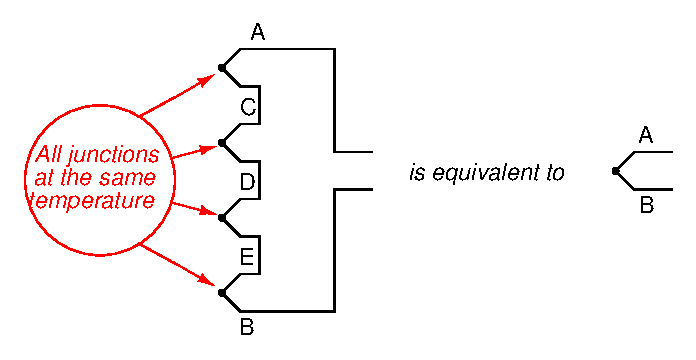
\includegraphics[width=15.5cm]{i00373x01.eps}$$

Med andre ord vil en skjøt mellom metall {\bf A} og {\bf B} gi samme spenning som en serie isotermiske skjøter {\bf A}-\textbf{C}, {\bf C}-\textbf{D}, {\bf D}-\textbf{E} og {\bf E}-\textbf{B}. Dette omtales ofte som loven om mellomliggende metaller.

Bruk dette prinsippet på kretsen under, og forenkle den slik at antall skjøter blir så lavt som mulig (anta at voltmeterledningene kan lages av valgfritt metall, så lenge begge er like):

$$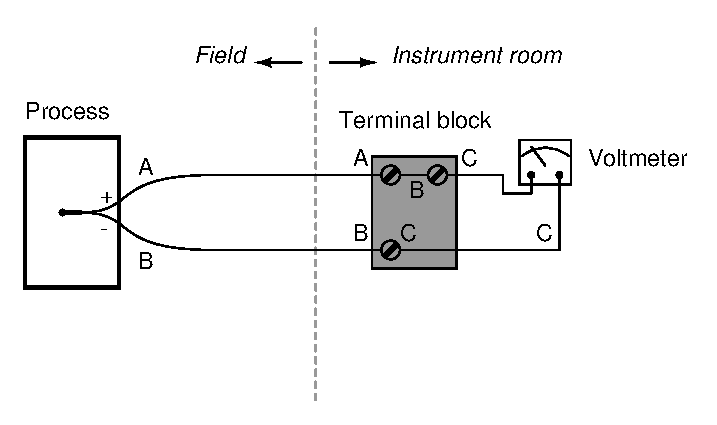
\includegraphics[width=15.5cm]{i00373x02.eps}$$

Vil termoelementet fungere likt dersom vi fjerner metallsegment {\bf B} ved terminalblokken? Forklar hvorfor eller hvorfor ikke.

$$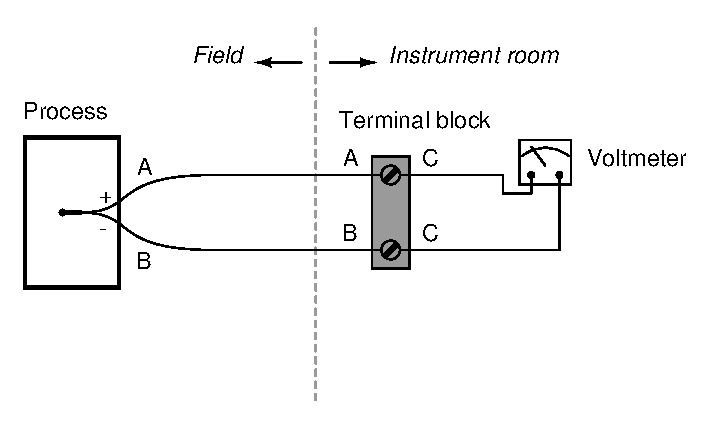
\includegraphics[width=15.5cm]{i00373x05.eps}$$

\underbar{file i00373}
%(END_QUESTION)





%(BEGIN_ANSWER)

Hvis begge voltmeterledningene lages av metall {\bf B}, kan skjøtene forenkles slik:

$$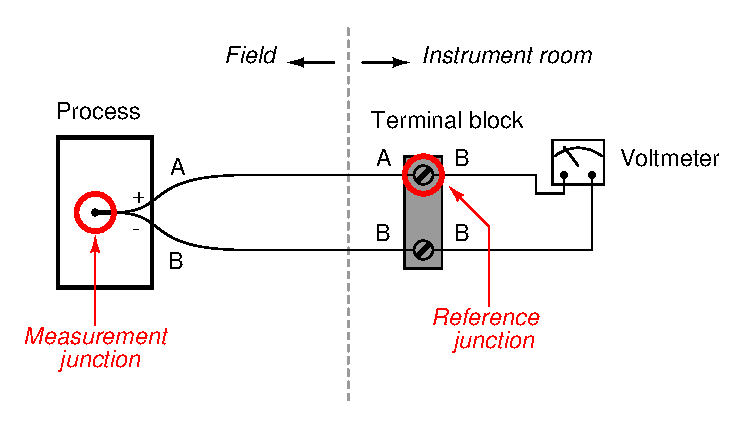
\includegraphics[width=15.5cm]{i00373x03.eps}$$

Å fjerne metall {\bf B} helt fungerer like godt. Da oppfører {\bf A-C}- og {\bf B-C}-skjøtene seg som én referanseskjøt, fordi de holdes ved samme temperatur av terminalblokkens varmeledning:

$$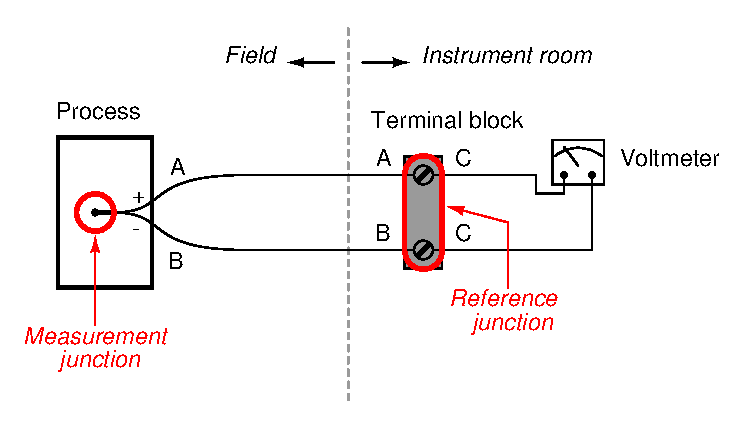
\includegraphics[width=15.5cm]{i00373x06.eps}$$

%(END_ANSWER)





%(BEGIN_NOTES)

Begge voltmeterledningene kunne også vært laget av metall {\bf A} med samme grad av forenkling. I begge tilfeller har sluttkretsen bare to skjøter mellom ulike metaller:

$$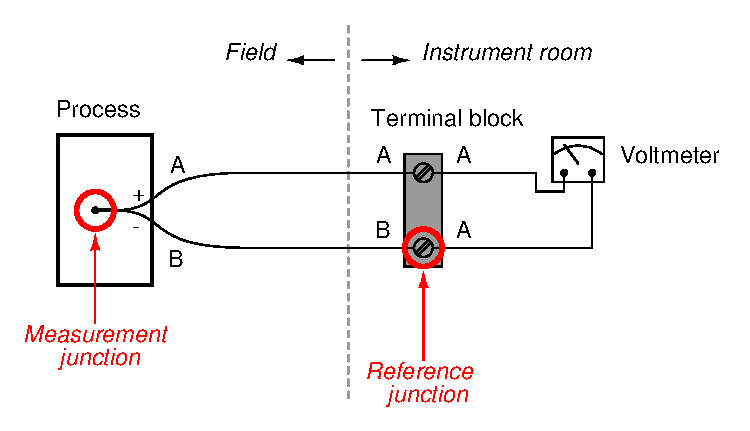
\includegraphics[width=15.5cm]{i00373x04.eps}$$

%INDEX% Measurement, temperature: thermocouple (law of intermediate metals)

%(END_NOTES)
